\documentclass[12pt, a4paper]{ctexart}

\usepackage{amsmath}
\usepackage{array}
\usepackage{appendix}
\usepackage{listings}
\usepackage{xcolor}
\usepackage{fontspec}
\usepackage{underscore}
\usepackage{graphicx}
\usepackage{subfigure}
\usepackage{multirow}
\setmonofont{Consolas}
\lstset{
	breaklines=true,
	language = C++, 
	numbers=left,
	backgroundcolor=\color{red!0!green!25!blue!25},%代码块背景色为浅灰色
	rulesepcolor= \color{gray}, %代码块边框颜色
	numberstyle= \small,%行号字体
	frame=shadowbox%用方框框住代码块
	frame=single
}

\title{间断有限元第五次作业报告}
\author{九所 $\quad$ 韩若愚}
\date{2022.5.10}
\begin{document}
	\maketitle
	
	\tableofcontents
	
	\section{题目}
	Code the following schemes for 
	\begin{equation*}
	\begin{cases}
	& u_t = u_{xx},\\
	& u(x,0) = \sin(x)
	\end{cases}
	\quad 0 \leq x \leq 2\pi
	\end{equation*}
	Take the final time as $T = 1$.
	
	1. bad DG scheme. Show pictures of the exact solution and the numerical solution.
	
	2. LDG method with the central flux. Show error tables.
	
	3. LDG method with alternating flux. Show error tables.
	
	\section{真解}
	
	不妨假设$u (x,t) = A(x)B(t)$,将之带入方程,得到:
	$$
	A \cdot B' = A'' \cdot B
	$$
	假设$A,B$不为0,则$B'/B = A''/A$。这个方程等号左边是只和$t$有关的函数,右边是只和$x$有关的函数,所以$B'/B = A''/A = c = const$。于是解两个常微分方程$B' = cB,\  A'' = cA$,且注意初值条件$ u(x,0) = A(x)B(0) = \sin(x)$,得到$B = exp(-t)$,$A = \sin(x)$。所以$u$为:
	$$
	u (x,t) = e^{-t} \sin(x).
	$$
	显然此时$u$满足方程,$u$是方程的真解。
	
	\section{算法}
	
	\subsection{bad DG}
	
	将方程$u_t = u_{xx}$看成:
	$$
	u_t - (u_x)_x = 0
	$$
	上面的方程显然是守恒形式,通量函数为:$f = u_x$。可以用之前求解守恒律使用的方法求解。
	
	先对单元$[0,2\pi]$ 进行均匀剖分。假设将区间均匀剖分为$n$份,令:
	\begin{equation*}
	0 = x_{\frac{1}{2}} < x_{\frac{3}{2}} < \dots < x_{n-\frac{1}{2}} < x_{n+\frac{1}{2}} = 2\pi
	\end{equation*}
	则第$j$个区间为:$ I_j = [x_{j- \frac{1}{2}}, x_{j + \frac{1}{2}}]$,记每个区间的长度都为$h = \frac{2\pi}{n},\  x_{j+1/2}^- = \lim_{x \in I_j, \, x \to x_{j+1/2}} \, x, \  x_{j+1/2}^+ = \lim_{x \in I_{j+1}, \, x \to x_{j+1/2}} \, x$。则此时DG格式为:
	
	求$u_h \in V_h^k$,$V_h^k = \{ v \, | \, v|_{I_j} \in P^k(I_j), \, \forall j = 1, \dots,n \}$,使得对$\forall v_h \in V_h^k, \  \forall j = 1,\dots,n$,都有:
	\begin{equation*}
	\int_{I_j} (u_h)_t v_h dx = - \int_{I_j} (u_h)_x (v_h)_x dx + \hat{u_x}_{j+1/2}(v_h)_{j+1/2}^- - \hat{u_x}_{j-1/2} (v_h)_{j-1/2}^+
	\end{equation*}
	其中$\hat{u_x}$为对$u_x$进行近似的数值通量。
	
	假设参考单元$I = [-1,1]$,在参考单元上取一组$P^k(I)$的基底$\{ \phi^l \}_{l=0}^k$,则通过同胚映射$ x = \frac{h}{2} (\xi + 1) + x_{j-1/2}$,能将$u_h$表示为:
	$$
	u_h(x) |_{I_j} = \sum_{l=0}^k u_j^l(t) \phi^l(\xi), \quad j = 1,\dots,n
	$$
	令$v_h = \phi^m, \  m = 1,\dots,n$,则DG格式变为:
	\begin{equation*}
	\begin{split}
	& \frac{h}{2} \sum_{l=0}^k (\int_{I_j} \phi^l \phi^m d\xi) \frac{d}{dt}u_j^l = - \frac{2}{h} \sum_{l=0}^k (\int_{I_j} \phi^l_{\xi} \phi^m_{\xi} d\xi) u_j^l\\
	& + \hat{u_x}_{j+1/2} \phi^m(1) - \hat{u_x}_{j-1/2} \phi^m(-1), \qquad j = 1, \dots, n
	\end{split}
	\end{equation*}
	在计算中取$\hat{u_x}_{j+1/2} = ((u_x)_{j+1/2}^+ + (u_x)_{j+1/2}^-)/2$,其中:$(u_x)_{j+1/2}^+ = \frac{2}{h}\sum_{l=0}^k u_{j+1}^l \phi^l_{\xi}(-1)$,$(u_x)_{j+1/2}^- = \frac{2}{h}\sum_{l=0}^k u_j^l \phi^l_{\xi}(1)$。
	
	在时间方向上使用SSPRK进行计算。
	
	\subsection{LDG}
	
	在LDG中引入了辅助变量$q$,方程变为:
	\begin{equation*}
	\begin{cases}
	& q = u_x\\
	& u_t = q_x
	\end{cases}
	\end{equation*}
	
	假设解空间$V_h^k$不变,则LDG为:求$q_h, u_h \in V_h^k$,使得对$\forall p_h, v_h \in V_h^K$,$\forall j = 1, \dots,n$,都有:
	\begin{equation*}
	\begin{cases}
	\int_{I_j} q_h p_h dx = & - \int_{I_j} u_h (p_h)_x dx + \hat{u}_{j+1/2} (p_h)_{j+1/2}^- - \hat{u}_{j-1/2} (p_h)_{j-1/2}^+\\
	\int_{I_j} (u_h)_t v_h dx = & - \int_{I_j} q_h (v_h)_x dx + \hat{q}_{j+1/2}(v_h)_{j+1/2}^- - \hat{q}_{j-1/2} (v_h)_{j-1/2}^+
	\end{cases}
	\end{equation*}
	
	设$u_h(x,t)|_{I_j} = \sum_{l=0}^k u_j^l(t) \phi^l(\xi(x))$,$q_h(x,t)|_{I_j} = \sum_{l=0}^k q_j^l(t) \phi^l(\xi(x))$,取$p_h = v_h = \phi^m,\  m = 1, \dots,n$,则方程为:
	\begin{equation*}
	\begin{cases}
	\frac{h}{2}\sum_{l=0}^k (\int_{I}\phi^l \phi^m d\xi) q_j^l = & - \sum_{l=0}^k (\int_I \phi^l (\phi^m)_{\xi} d\xi) u_j^l \\
		& \qquad + \hat{u}_{j+1/2} \phi^m(1) - \hat{u}_{j-1/2} \phi^m(-1)\\
	\frac{h}{2} \sum_{l=0}^k (\int_I \phi^l \phi^m d\xi) \frac{d}{dt}u_j^l = & - \sum_{l=0}^k (\int_I \phi^l (\phi^m)_{\xi} d\xi) q_j^l \\
		& \qquad + \hat{q}_{j+1/2} \phi^m(1) - \hat{q}_{j-1/2} \phi^m(-1)
	\end{cases}
	\end{equation*}
	在第$m$次计算时,$u_h$的系数矩阵$(u_j^l)$是已知的,所以可以算出$q_h$的系数矩阵$(q_j^l)$,再用$(q_j^l)$通过SSPRK求解下一时刻$u_h$的系数。
	
	数值通量$\hat{q}_{j+1/2}, \  \hat{u}_{j+1/2}$可以选择成:
	
	1. 中心通量:$\hat{q}_j+1/2 = \frac{1}{2} (q_{j+1/2}^+ + q_{j+1/2}^-)$,$\hat{u}_j+1/2 = \frac{1}{2} (u_{j+1/2}^+ + u_{j+1/2}^-)$
	
	2. 交错通量:$\hat{q}_{j+1/2} = q_{j+1/2}^+$,$\hat{u}_{j+1/2} = u_{j+1/2}^-$。
	
	\section{数值结果}
	
	\subsection{bad DG}
	
	利用bad DG求解得到的数值结果图像见图\ref{1}。其中数值解在第$j$个点的值取为$u_h$在$x_j = (x_{j-1/2} + x_{j+1/2})/2$处的值。
	
	\begin{figure}[htbp]
		\centering
		\subfigure[$P^1$]{
			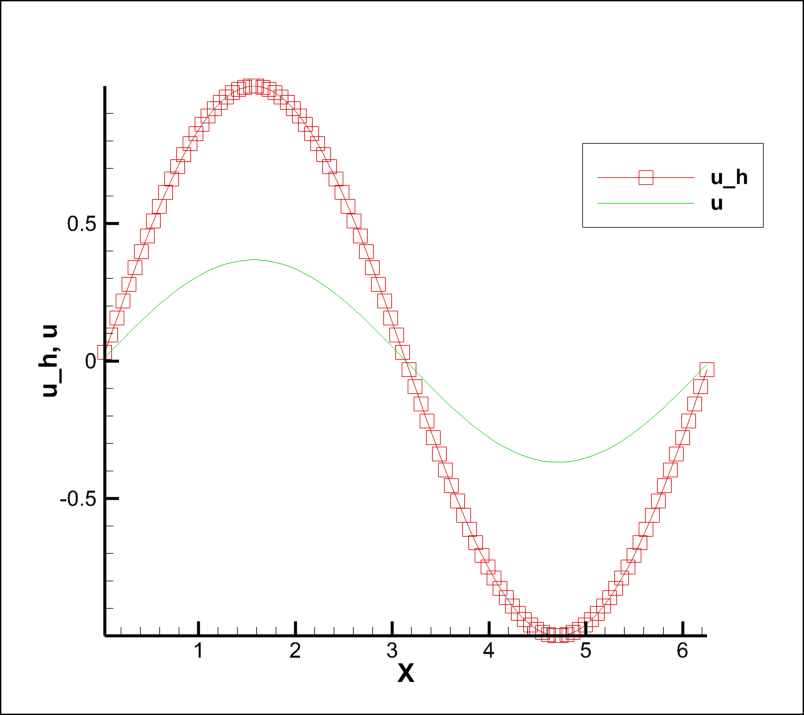
\includegraphics[width=5cm]{pics/badDGP1flux2.png}
		}
		\quad
		\subfigure[$P^2$]{
			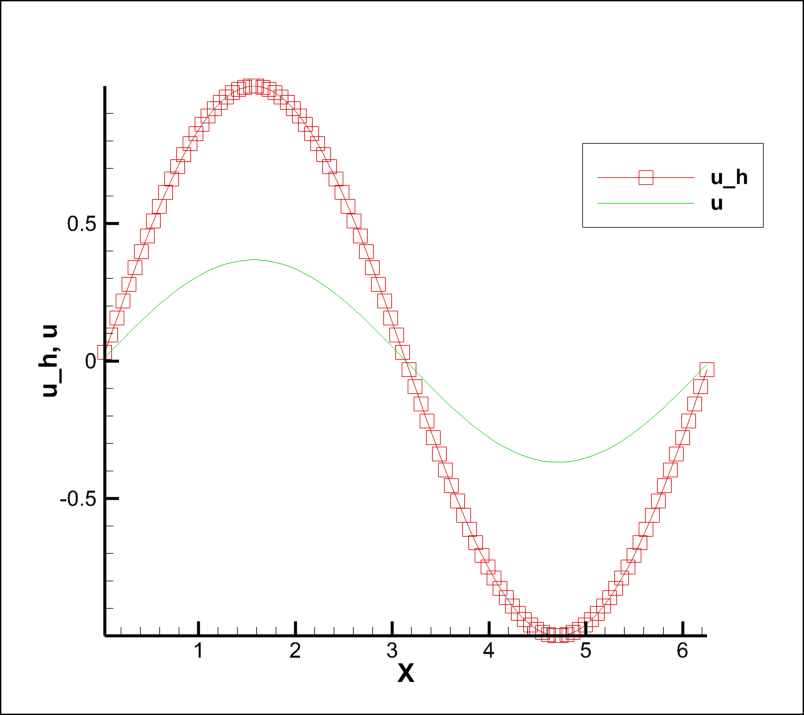
\includegraphics[width=5cm]{pics/badDGP2flux2.png}
		}
		\caption{bad DG at $T=1$}
		\label{1}
	\end{figure}

	\subsection{LDG}
	
	利用LDG求解得到的误差表见表\ref{2}、表\ref{3},保留三位小数。
	\begin{table}[htbp]
		\centering
		\caption{$P^1$}
		\label{2}
		\begin{tabular}{| p{50pt}<{\centering} | p{60pt}<{\centering} | p{60pt}<{\centering} || p{60pt}<{\centering} | p{60pt}<{\centering}|}
			\hline
			\multicolumn{5}{|c|}{LDG with central flux} \\
			\hline
			n & $L^2$ error & order & $L^\infty$error & order \\
			\hline
			20 & 1.505e-2 &  & 1.449e-2 &  \\
			\hline
			40 & 7.424e-3 & 1.019 & 7.226e-3 & 1.004\\
			\hline
			80 & 3.699e-3 & 1.005 & 3.611e-3 & 1.009\\
			\hline
			160 & 1.848e-3 & 1.001 & 1.805e-3 & 1.000\\
			\hline
			320 & 9.239e-4 & 1.000 & 9.026e-4 & 1.000\\
			\hline
			\multicolumn{5}{|c|}{LDG with alternating flux} \\
			\hline
			n & $L^2$ error & order & $L^\infty$error & order \\
			\hline
			20 & 3.922e-3 &  & 6.010e-3 &  \\
			\hline
			40 & 9.794e-4 & 2.002 & 1.510e-3 & 1.993\\
			\hline
			80 & 2.448e-4 & 2.000 & 3.780e-4 & 1.998\\
			\hline
			160 & 6.120e-5 & 2.000 & 9.453e-5 & 2.000\\
			\hline
			320 & 1.530e-5 & 2.000 & 2.363e-5 & 2.000\\
			\hline
		\end{tabular}
	\end{table}

	\begin{table}[htbp]
		\centering
		\caption{$P^2$}
		\label{3}
		\begin{tabular}{| p{50pt}<{\centering} | p{60pt}<{\centering} | p{60pt}<{\centering} || p{60pt}<{\centering} | p{60pt}<{\centering}|}
			\hline
			\multicolumn{5}{|c|}{LDG with central flux} \\
			\hline
			n & $L^2$ error & order & $L^\infty$error & order \\
			\hline
			20 & 6.442e-5 &  & 9.650e-5 &  \\
			\hline
			40 & 7.983e-6 & 3.013 & 1.195e-5 & 3.014\\
			\hline
			80 & 9.962e-7 & 3.002 & 1.506e-6 & 2.988\\
			\hline
			160 & 1.245e-7 & 3.000 & 1.896e-7 & 2.990\\
			\hline
			320 & 1.565e-8 & 2.992 & 2.386e-8 & 2.990\\
			\hline
			\multicolumn{5}{|c|}{LDG with alternating flux} \\
			\hline
			n & $L^2$ error & order & $L^\infty$error & order \\
			\hline
			20 & 9.866e-5 &  & 1.886e-4 &  \\
			\hline
			40 & 1.233e-5 & 3.000 & 2.374e-5 & 2.990\\
			\hline
			80 & 1.542e-6 & 2.999 & 2.989e-6 & 2.990\\
			\hline
			160 & 1.934e-7 & 2.995 & 3.910e-7 & 2.934\\
			\hline
			320 & 2.434e-8 & 2.990 & 5.120e-8 & 2.933\\
			\hline
		\end{tabular}
	\end{table}

	\newpage
	\section{分析}
	
	图\ref{1}显示当使用bad DG时,得到的数值结果和真解并不相符,产生这种问题的原因是这个格式并不稳定。所以bad DG并不是求解对流扩散方程的好方法。使用LDG能得到符合真解的结果。LDG的结果会受到通量函数的选取的影响。当使用中心通量时,在$k=1$的情况下使用中心通量时$L^1$和$L^\infty$范数下的收敛阶为1阶,但是使用交错通量时收敛阶是2阶。当$k=2$时无论哪个收敛阶都保持在3阶左右。
	
	\section{代码}
	本次报告程序使用C++编译。
	
	\appendix
	
	\begin{lstlisting}
	#include <iostream>
	#include <cmath>
	#include <fstream>
	using namespace std;
	
	
	//************部分参数**************//
	const int n = 320;   //划分单元个数
	const int k = 2;    //多项式最高次项次数
	
	const double pi = 3.1415926;
	const double h = 2 * pi / n;    //空间步长
	double dt = 1e-5 ;    //时间步长
	double p[n+1];  //节点位置,p_j = j * h = x_{j+1/2}, j =0,1, ..., n
	
	const double lobattopoint[5] = {-1.0, -0.6546536707079771, 0, 0.6546536707079771, 1.0};
	const double lobattoco[5] = {0.1, 0.5444444444444444, 0.7111111111111111, 0.5444444444444444, 0.1};
	//*************参数定义完毕*********//
	
	//*************函数声明*************//
	double u_0(double x);   //初值
	double u_exact(double x, double t);   //真解
	double phi(int l, double x);    //参考单元基函数
	double phix(int l, double x);   //基函数一阶导
	double** initial();   //计算初始时刻u_j
	double fluxu(double ul, double ur);  //数值通量计算
	double fluxq(double ql, double qr);
	void getq(double ut);
	double** L(double** ut);   //用于计算RK的函数,u_t= F(u)
	double** RK22(double** un, double dtn);    //2步二阶RK
	double** RK33(double** un, double dtn);
	double** RK(int k, double** un, double dtn);
	//************声明完毕**************//
	
	
	int main()
	{
	int i, j, l;
	double t, temp1, temp2, norm1, norm2, xi;
	double T = 1;
	double** u1 = new double* [n];
	double** u2 = new double* [n];
	for (i=0; i<n; i++)
	{
	u1[i] = new double [k+1];
	u2[i] = new double [k+1];
	}
	for (j=0; j<=n; j++)
	{
	p[j] = j * h;
	}
	
	u1 = initial();
	t = 0;
	while(t<T)
	{
	if ( t + dt >T)
	{
	dt = T - t;
	}
	t = t + dt;
	u2 = RK(k,u1,dt);
	u1 = u2;
	cout<<"t="<<t<<endl;
	}
	
	//计算误差
	norm1 = 0;
	norm2 = 0;
	for (j=1; j<=n; j++)
	{
	for (i=0; i<5; i++)
	{
	xi = lobattopoint[i];
	temp1 = 0;
	for (l=0; l<=k; l++)
	{
	temp1 = temp1 + u1[j-1][l] * phi(l,xi);
	}
	
	temp2 = h * (xi + 1) / 2. + p[j-1];
	temp1 = u_exact(temp2,T) - temp1;
	
	if (abs(temp1) > norm2)
	{
	norm2 = abs(temp1);
	}
	
	temp1 = temp1 * temp1;
	norm1 = norm1 + lobattoco[i] * temp1;
	}
	
	}
	norm1 = norm1 * h / 2.;
	norm1 = sqrt(norm1);
	cout<<"L2="<<norm1<<endl<<"Linf="<<norm2<<endl;//*/
	
	//开始画图
	{
	const char* fn = "DGLecture\\homework5\\LDG.plt";
	remove(fn);
	fstream f, f1;
	f.open(fn, ios::out | ios :: app);
	f<<"VARIABLES="<<"X"<<","<<"u_h"<<","<<"u"<<endl;
	for (j=1; j<=n; j++)
	{
	temp1 = 0;
	for (l=0; l<=k; l++)
	{
	temp1 = temp1 + u1[j-1][l] * phi(l,0);
	}
	f<<"\t"<<(p[j-1] + p[j])/2.0<<"\t"<<temp1<<"\t"<<u_exact((p[j-1] + p[j])/2.0,T)<<endl;
	
	}
	f.close();
	}
	
	for (i=0; i<n; i++)
	{
	delete[] u1[i];
	delete[] u2[i];
	}
	delete[] u1;
	delete[] u2;
	
	system("pause");
	}
	
	//**********函数定义***********//
	
	double u_0(double x)
	{
	return sin(x);
	}
	
	double u_exact(double x, double t)
	{
	double ans;
	ans = exp(-t) * sin(x);
	return ans;
	}
	
	double phi(int l, double x)
	{
	if (l==0)
	{
	return 1;
	}
	else if (l == 1)
	{
	return x;
	}
	else if (l == 2)
	{
	return (3*x*x - 1)/2;
	}
	else{
	return 0;
	}
	}
	
	double** initial()
	{
	double ans, temp;
	int j, l, m;
	double** ut = new double* [n];
	double* Bt = new double [n];
	for (j=0; j<n; j++)
	{
	ut[j] = new double [k+1];
	}
	
	for (j=1; j<=n; j++)
	{
	for (m=0; m<=k; m++)
	{
	ans = 0;
	for (l=0; l<5; l++)
	{
	temp = h * (lobattopoint[l] + 1)/2 + p[j-1];
	ans = ans + lobattoco[l] * u_0(temp) * phi(m,lobattopoint[l]);
	}
	ans = ans / 2;
	Bt[m] = ans;
	}
	
	double A[3][3] = {{1,0,0},{0,3,0},{0,0,5}};
	for (m=0; m<=k ;m++)
	{
	ut[j-1][m] = 0;
	for (l=0; l<=k; l++)
	{
	ut[j-1][m] = ut[j-1][m] + A[m][l] * Bt[l];
	}
	} 
	}
	delete[] Bt;
	return ut;
	}
	
	double fluxu(double ul, double ur)
	{
	double ans;
	//average flux
	//ans = 0.5 * (ul + ur);
	
	//alternating flux
	ans = ul;
	
	return ans;
	}
	
	double fluxq(double ql, double qr)
	{
	double ans;
	//average flux
	//ans = 0.5 * (ql + qr);
	
	//alternating flux
	ans = qr;
	
	return ans;
	}
	
	double** getq(double** ut)
	{
	int j, l, m, r;
	double ul, ur;
	double** q = new double* [n];
	for (j=0; j<n; j++)
	{
	q[j] = new double [k+1];
	}
	
	double A[3] = {1,3,5};
	double B[3][3] = {{0,0,0},{2,0,0},{0,2,0}};
	
	for ( j=1; j<=n; j++)
	{
	for (m=0; m<=k; m++)
	{
	q[j-1][m] = 0;
	
	for (l=0; l<=k; l++)
	{
	q[j-1][m] = q[j-1][m] - B[m][l] * ut[j-1][l];
	}
	//第一个数值通量
	{
	ul = 0;
	ur = 0;
	
	r = j;
	if (r == n)
	{
	r = 0;
	}
	for (l=0; l<=k; l++)
	{
	ul = ul + ut[j-1][l] * phi(l,1);
	ur = ur + ut[r][l] * phi(l,-1);
	}
	
	q[j-1][m] = q[j-1][m] + fluxu(ul, ur) * phi(m,1);
	}
	//第二个数值通量
	{
	ul = 0;
	ur = 0;
	
	r = j-2;
	if (r == -1)
	{
	r = n-1;
	}
	for (l=0; l<=k; l++)
	{
	ul = ul + ut[r][l] * phi(l,1);
	ur = ur + ut[j-1][l] * phi(l,-1);
	}
	
	q[j-1][m] = q[j-1][m] - fluxu(ul, ur) * phi(m,-1);
	}
	q[j-1][m] = q[j-1][m] * A[m] / h;
	}
	}
	
	return q;
	}
	
	double** L(double** ut)
	{
	int i, j, l, m, p;
	double ql, qr;
	double** ans = new double* [n];
	double** q = new double* [n];
	for (i=0; i<n; i++)
	{
	ans[i] = new double [k+1];
	q[i] = new double [k+1];
	}
	q = getq(ut);
	
	double A[3] = {1,3,5};
	double B[3][3] = {{0,0,0},{2,0,0},{0,2,0}};
	
	for (j=1; j<=n; j++)
	{
	for (m=0; m<=k; m++)
	{
	ans[j-1][m] = 0;
	
	for (l=0; l<=k; l++)
	{
	ans[j-1][m] = ans[j-1][m] - B[m][l] * q[j-1][l];
	}
	
	//第一个数值通量
	{
	p = j;
	if (p == n)
	{
	p = 0;
	}
	
	ql = 0;
	qr = 0;
	
	for (l=0; l<=k; l++)
	{
	ql = ql + q[j-1][l] * phi(l,1);
	qr = qr + q[p][l] * phi(l,-1);
	}
	
	ans[j-1][m] = ans[j-1][m] + fluxq(ql,qr) * phi(m,1);
	}
	//第二个数值通量
	{
	p = j-2;
	if (p == -1)
	{
	p = n-1;
	}
	
	ql = 0;
	qr = 0;
	
	for (l=0; l<=k; l++)
	{
	ql = ql + q[p][l] * phi(l,1);
	qr = qr + q[j-1][l] * phi(l,-1);
	}
	
	ans[j-1][m] = ans[j-1][m] - fluxq(ql,qr) * phi(m,-1);
	}
	ans[j-1][m] = ans[j-1][m] * A[m] / h;
	}
	
	}
	for (i=0; i<n; i++)
	{
	delete[] q[i];
	}
	delete[] q;
	return ans;
	}
	
	double** RK22(double** un, double dtn)
	{
	int j,l,m;
	double ul;
	double** ans = new double* [n];
	for (j=0; j<n; j++)
	{
	ans[j] = new double [k+1];
	}
	double** u0 = new double* [n];
	double** u1 = new double* [n];
	double** u2 = new double* [n];
	
	for (j=0; j<n; j++)
	{
	u0[j] = new double [k+1];
	u1[j] = new double [k+1];
	u2[j] = new double [k+1];
	}
	
	for (j=1; j<=n; j++)
	{
	for (l=0; l<=k; l++)
	{
	u0[j-1][l] = un[j-1][l];
	}
	}
	
	u1 = L(u0);
	for (j=1; j<=n; j++)
	{
	for (l=0; l<=k; l++)
	{
	u1[j-1][l] = u1[j-1][l] * dtn  + u0[j-1][l];
	}
	}
	
	u2 = L(u1);
	for (j=1; j<=n;j++)
	{
	for (l=0; l<=k; l++)
	{
	u2[j-1][l] = u0[j-1][l] * 0.5 + u1[j-1][l] * 0.5 + u2[j-1][l] * 0.5 * dtn;
	ans[j-1][l] = u2[j-1][l];
	}
	}
	
	delete[] u0;
	delete[] u1;
	delete[] u2;
	
	return ans;
	}
	
	double** RK33(double** un, double dtn)
	{
	int j,l,m;
	double ul;
	double** ans = new double* [n];
	for (j=0; j<n; j++)
	{
	ans[j] = new double [k+1];
	}
	double** u0 = new double* [n];
	double** u1 = new double* [n];
	double** u2 = new double* [n];
	double** u3 = new double* [n];
	
	for (j=0; j<n; j++)
	{
	u0[j] = new double [k+1];
	u1[j] = new double [k+1];
	u2[j] = new double [k+1];
	u3[j] = new double [k+1];
	}
	
	for (j=1; j<=n; j++)
	{
	for (l=0; l<=k; l++)
	{
	u0[j-1][l] = un[j-1][l];
	}
	}
	
	u1 = L(u0);
	for (j=1; j<=n; j++)
	{
	for (l=0; l<=k; l++)
	{
	u1[j-1][l] = u1[j-1][l] * dtn  + u0[j-1][l];
	}
	}
	
	u2 = L(u1);
	for (j=1; j<=n;j++)
	{
	for (l=0; l<=k; l++)
	{
	u2[j-1][l] = u0[j-1][l] * 3 / 4.0 + u1[j-1][l] /4 + u2[j-1][l] * dtn / 4.0;
	}
	}
	
	u3 = L(u2);
	for (j=1; j<=n; j++)
	{
	for (l=0; l<=k; l++)
	{
	u3[j-1][l] = u0[j-1][l] / 3.0 + 2 * u2[j-1][l] / 3.0 + 2 * dtn * u3[j-1][l] /3.0;
	ans[j-1][l] = u3[j-1][l];
	}
	}
	
	delete[] u0;
	delete[] u1;
	delete[] u2;
	delete[] u3;
	
	return ans;
	}
	
	double** RK(int k, double** un, double dtn)
	{
	double** u2;
	if ( k == 1 )
	{
	u2 = RK22(un,dtn);
	}
	else if (k == 2)
	{
	u2 = RK33(un,dtn);
	}
	else{
	;
	}
	
	return u2;
	}
	\end{lstlisting}
	
	
\end{document}